\documentclass{article}
\usepackage[margin=1in]{geometry}
\usepackage[linesnumbered,ruled,vlined]{algorithm2e}
\usepackage{amsfonts}
\usepackage{amsmath}
\usepackage{amssymb}
\usepackage{amsthm}
\usepackage{enumitem}
\usepackage{fancyhdr}
\usepackage{hyperref}
\usepackage{minted}
\usepackage{multicol}
\usepackage{pdfpages}
\usepackage{standalone}
\usepackage[many]{tcolorbox}
\usepackage{tikz-cd}
\usepackage{transparent}
\usepackage{xcolor}
% \tcbuselibrary{minted}

\author{Nathan Solomon}

\newcommand{\fig}[1]{
    \begin{center}
        \includegraphics[width=\textwidth]{#1}
    \end{center}
}

% Math commands
\renewcommand{\d}{\mathrm{d}}
\DeclareMathOperator{\id}{id}
\DeclareMathOperator{\im}{im}
\DeclareMathOperator{\proj}{proj}
\DeclareMathOperator{\Span}{span}
\DeclareMathOperator{\Tr}{Tr}
\DeclareMathOperator{\tr}{tr}
\DeclareMathOperator{\ad}{ad}
\DeclareMathOperator{\ord}{ord}
%%%%%%%%%%%%%%% \DeclareMathOperator{\sgn}{sgn}
\DeclareMathOperator{\Aut}{Aut}
\DeclareMathOperator{\Inn}{Inn}
\DeclareMathOperator{\Out}{Out}
\DeclareMathOperator{\stab}{stab}

\newcommand{\N}{\ensuremath{\mathbb{N}}}
\newcommand{\Z}{\ensuremath{\mathbb{Z}}}
\newcommand{\Q}{\ensuremath{\mathbb{Q}}}
\newcommand{\R}{\ensuremath{\mathbb{R}}}
\newcommand{\C}{\ensuremath{\mathbb{C}}}
\renewcommand{\H}{\ensuremath{\mathbb{H}}}
\newcommand{\F}{\ensuremath{\mathbb{F}}}

\newcommand{\E}{\ensuremath{\mathbb{E}}}
\renewcommand{\P}{\ensuremath{\mathbb{P}}}

\newcommand{\es}{\ensuremath{\varnothing}}
\newcommand{\inv}{\ensuremath{^{-1}}}
\newcommand{\eps}{\ensuremath{\varepsilon}}
\newcommand{\del}{\ensuremath{\partial}}
\renewcommand{\a}{\ensuremath{\alpha}}

\newcommand{\abs}[1]{\ensuremath{\left\lvert #1 \right\rvert}}
\newcommand{\norm}[1]{\ensuremath{\left\lVert #1\right\rVert}}
\newcommand{\mean}[1]{\ensuremath{\left\langle #1 \right\rangle}}
\newcommand{\floor}[1]{\ensuremath{\left\lfloor #1 \right\rfloor}}
\newcommand{\ceil}[1]{\ensuremath{\left\lceil #1 \right\rceil}}
\newcommand{\bra}[1]{\ensuremath{\left\langle #1 \right\rvert}}
\newcommand{\ket}[1]{\ensuremath{\left\lvert #1 \right\rangle}}
\newcommand{\braket}[2]{\ensuremath{\left.\left\langle #1\right\vert #2 \right\rangle}}

\newcommand{\catname}[1]{{\normalfont\textbf{#1}}}

\newcommand{\up}{\ensuremath{\uparrow}}
\newcommand{\down}{\ensuremath{\downarrow}}

% Custom environments
\newtheorem{thm}{Theorem}[section]

\definecolor{probBackgroundColor}{RGB}{250,240,240}
\definecolor{probAccentColor}{RGB}{140,40,0}
\newenvironment{prob}{
    \stepcounter{thm}
    \begin{tcolorbox}[
        boxrule=1pt,
        sharp corners,
        colback=probBackgroundColor,
        colframe=probAccentColor,
        borderline west={4pt}{0pt}{probAccentColor},
        breakable
    ]
    \color{probAccentColor}\textbf{Problem \thethm.} \color{black}
} {
    \end{tcolorbox}
}

\definecolor{exampleBackgroundColor}{RGB}{212,232,246}
\newenvironment{example}{
    \stepcounter{thm}
    \begin{tcolorbox}[
      boxrule=1pt,
      sharp corners,
      colback=exampleBackgroundColor,
      breakable
    ]
    \textbf{Example \thethm.}
} {
    \end{tcolorbox}
}

\definecolor{propBackgroundColor}{RGB}{255,245,220}
\definecolor{propAccentColor}{RGB}{150,100,0}
\newenvironment{prop}{
    \stepcounter{thm}
    \begin{tcolorbox}[
        boxrule=1pt,
        sharp corners,
        colback=propBackgroundColor,
        colframe=propAccentColor,
        breakable
    ]
    \color{propAccentColor}\textbf{Proposition \thethm. }\color{black}
} {
    \end{tcolorbox}
}

\definecolor{thmBackgroundColor}{RGB}{235,225,245}
\definecolor{thmAccentColor}{RGB}{50,0,100}
\renewenvironment{thm}{
    \stepcounter{thm}
    \begin{tcolorbox}[
        boxrule=1pt,
        sharp corners,
        colback=thmBackgroundColor,
        colframe=thmAccentColor,
        breakable
    ]
    \color{thmAccentColor}\textbf{Theorem \thethm. }\color{black}
} {
    \end{tcolorbox}
}

\definecolor{corBackgroundColor}{RGB}{240,250,250}
\definecolor{corAccentColor}{RGB}{50,100,100}
\newenvironment{cor}{
    \stepcounter{thm}
    \begin{tcolorbox}[
        enhanced,
        boxrule=0pt,
        frame hidden,
        sharp corners,
        colback=corBackgroundColor,
        borderline west={4pt}{0pt}{corAccentColor},
        breakable
    ]
    \color{corAccentColor}\textbf{Corollary \thethm. }\color{black}
} {
    \end{tcolorbox}
}

\definecolor{lemBackgroundColor}{RGB}{255,245,235}
\definecolor{lemAccentColor}{RGB}{250,125,0}
\newenvironment{lem}{
    \stepcounter{thm}
    \begin{tcolorbox}[
        enhanced,
        boxrule=0pt,
        frame hidden,
        sharp corners,
        colback=lemBackgroundColor,
        borderline west={4pt}{0pt}{lemAccentColor},
        breakable
    ]
    \color{lemAccentColor}\textbf{Lemma \thethm. }\color{black}
} {
    \end{tcolorbox}
}

\definecolor{proofBackgroundColor}{RGB}{255,255,255}
\definecolor{proofAccentColor}{RGB}{80,80,80}
\renewenvironment{proof}{
    \begin{tcolorbox}[
        enhanced,
        boxrule=1pt,
        sharp corners,
        colback=proofBackgroundColor,
        colframe=proofAccentColor,
        borderline west={4pt}{0pt}{proofAccentColor},
        breakable
    ]
    \color{proofAccentColor}\emph{\textbf{Proof. }}\color{black}
} {
    \qed \end{tcolorbox}
}

\definecolor{noteBackgroundColor}{RGB}{240,250,240}
\definecolor{noteAccentColor}{RGB}{30,130,30}
\newenvironment{note}{
    \begin{tcolorbox}[
        enhanced,
        boxrule=0pt,
        frame hidden,
        sharp corners,
        colback=noteBackgroundColor,
        borderline west={4pt}{0pt}{noteAccentColor},
        breakable
    ]
    \color{noteAccentColor}\textbf{Note. }\color{black}
} {
    \end{tcolorbox}
}


\fancyhf{}
\setlength{\headheight}{24pt}

\date{\today}
\title{MATH 131B Homework \#3}

\begin{document}
\maketitle

\begin{prob}
    3.1.2. Prove proposition 3.1.5.
\end{prob}
\fbox{$(a) \Leftrightarrow (b)$} By the definitions of limits and of convergence, both (a) and (b) are equivalent to the statement that for any $\varepsilon/ > 0$, there exists $\delta > 0$ such that whenever $d(x, x_0) < \delta, x \in E$, $d(f(x), L) < \epsilon$.
\par
\fbox{$(b) \Rightarrow (c)$} 

\bigskip
\begin{prob}
    3.1.5
\end{prob}
This question is phrased weirdly, so I will assume that $E$ is a subset of $X$, and that the statement we want to prove is $\lim_{x \rightarrow x_0, x \in E} g \circ f (x) = z_0$ (instead of $\lim_{x \in x_0, x \in E} g \circ f (x) = z_0$).
\par
For any $\varepsilon > 0$, there exists $\delta > 0$ such that $B(y_0, \delta) \subset g^{-1}(B(z_0, \varepsilon))$, and there also exists $\gamma > 0$ such that $B(x_0, \gamma) \subset f^{-1}(B(y_0, \delta))$. We have found a positive $\gamma$ such that $B(x_0, \gamma) \subset (g \circ f)^{-1}(B(z_0, \varepsilon))$, so $\lim_{x \rightarrow x_0, x \in E} g \circ f (x) = z_0$.

\bigskip
\begin{prob}
    3.2.1
\end{prob}
\textbf{Part (a).} If $f$ is continuous, then at each $x_0 \in \R$, for every $\varepsilon > 0$, there exists $\delta > 0$ such that whenever $d(x, x_0) < \delta$, $d(f(x), f(x_0)) < \varepsilon$. If $a_n$ converges to zero, there exists $N \in \N$ such that for any $n \geq N$, $d(a_n, 0) < \delta$. So for any $n \geq N$, $f_{a_n}(x_0) = f(x_0 - a_n)$ which is equal to $f(x)$ for some $x$ such that $d(x, x_0) < \delta$. That implies $d(f(x), f(x_0)) < \varepsilon$, so $d(f_{a_n}(x_0), f(x_0)) < \varepsilon$. Since this works at any $x_0 \in \R$, the shifted functions $f_{a_n}$ converge pointwise to $f$.
\par
If the shifted functions converge pointwise to $f$ (for ANY sequence $a_n$ which converges to 0), then suppose for the sake of contradiction that $f$ is not continuous. That would mean there is $x_0 \in X, \varepsilon > 0$ such that there is no $\delta > 0$ for which $f(B(x_0, \delta)) \subset B(f(x_0), \varepsilon)$. Then for each $n \in \N$, let $a_n$ be a number in $B(x_0, \delta)$ such that $d(f(x_0), f(x_0-a)) \geq \varepsilon$. $a_n$ is a sequence which converges to zero, but for which $f_{a_n}(x_0)$ does not converge to zero.
\par
\textbf{Part (b).} If $f$ is continuous, then for every $\varepsilon > 0$, there exists $\delta > 0$ such that at any $x_0$, whenever $d(x, x_0) < \delta$, $d(f(x), f(x_0)) < \varepsilon$. If $a_n$ converges to zero, there exists $N \in \N$ such that for any $n \geq N$, $d(a_n, 0) < \delta$. So for any $n \geq N$, $f_{a_n}(x_0) = f(x_0 - a_n)$ which is equal to $f(x)$ for some $x$ such that $d(x, x_0) < \delta$. That implies $d(f(x), f(x_0)) < \varepsilon$, so $d(f_{a_n}(x_0), f(x_0)) < \varepsilon$. Therefore the shifted functions $f_{a_n}$ converge uniformly to $f$.
\par
If the shifted functions $f_{a_n}$ converge uniformly to $f$ (for any sequence $a_n$ which converges to 0), then suppose for the sake of contradiction that $f$ is not uniformly continuous. That would mean there exists some $\varepsilon > 0$ such that there is no $\delta > 0$ such that whenever $d(x_1, x_2) < \delta$, $d(f(x_1), f(x_2)) < \varepsilon$. That means there exists some $\varepsilon > 0$ such that for any $n \in \N$, there exist $x^{(n)}_1, x^{(n)}_2 \in X$ satisfying $d(x^{(n)}_1, x^{(n)}_2) < \frac{1}{n}$ and $d(f(x^{(n)}_1), f(x^{(n)}_2)) \geq \varepsilon$. Let $a_n = x^{(n)}_1 - x^{(n)}_2$. Then for any $n$, $d(f(x^{(n)}_1), f_{a_n}(x^{(n)}_1)) \geq \varepsilon$, so the shifted functions do not converge uniformly to $f$, which contradicts our assumption.

\bigskip
\begin{prob}
    3.2.2.ab
\end{prob}
\textbf{Part (a).} If $f^{(n)}$ converges uniformly to $f$, then for any $\varepsilon > 0$, there exists $N(\varepsilon) \in \N$ such that for any $n \geq N(\varepsilon)$ and any $x \in X$, $d(f_n(x), f(x)) < \varepsilon$. So for any $\varepsilon > 0$ and any $x_0 \in X$, let $N(\varepsilon, x_0)$ be equal to that same $N(\varepsilon)$. Then for any $n \geq N(\varepsilon, x_0)$, $d(f_n(x_0), f(x_0)) < \varepsilon$, so $f_n$ converges pointwise to $f$.
\par
\textbf{Part (b).} For any $x_0 \in (-1, 1)$ and any $\varepsilon > 0$, let $N = \ceil{\log{\varepsilon} / \log{\abs{x_0}}}$. Then for any $n \geq N$,
\begin{align*}
\abs{f^{(n)}(x_0)} &= \abs{x_0}^n \\
                   &= \abs{x_0}^{\ceil{\log{\varepsilon} / \log{\abs{x_0}}}} \\
                   &\leq \abs{x_0}^{\log \varepsilon / \log \abs{x_0}} \\
                   &= \exp \left( \frac{\log\abs{x_0} \log\varepsilon}{\log \abs{x_0}} \right) \\
                   &= \varepsilon \\
d(f^{(n)}(x_0), 0) &\leq \varepsilon.
\end{align*}
Therefore $f^{(n)}$ converges pointwise to the zero function.
\par
Now define $f^{(n)'}$ so that the domain is $(-1, 1]$ (and it also maps $x$ to $x^n$). These converge to a function $f': (-1, 1] \rightarrow \R$ which maps $1$ to $1$ and every other point to zero. However, that convergence is not uniform, because a sequence of continuous functions cannot converge uniformly to a discontinuous function. Since the convergence is not uniform, there exists some $\varepsilon > 0$ such that for any $\delta > 0$, for arbitrarily large $n$, you can find $x_1, x_2 \in (-1, 1]$ such that $x_1 < x_2$, $d(x_1, x_2) < \delta$, and $d(f^{(n)'}(x_1), f^{(n)'}(x_2)) > 2\varepsilon$. Since $f^{(n)'}$ is continuous, you could also find $x_3$ (for arbitrarily large $n$) such that $x_1 < x_3 < x_2$ and $d(f^{(n)'}(x_2), f^{(n)'}(x_3)) < \varepsilon$, so by the triangle inequality $d(f^{(n)'}(x_1), f^{(n)'}(x_3)) > \varepsilon$. $x_1$ and $x_3$ are both in $(-1, 1)$, so even if we restricted the domain to $(-1, 1)$, this would still prove that the sequence of functions doesn't converge uniformly to $f$.

\bigskip
\begin{prob}
    3.2.4
\end{prob}
We are given that $f$ is bounded, meaning there exists $r \in \R$ such that for any $x \in X$, $d(f(x), y_0) < r$. For any $\varepsilon > 0$, there exists $N \in \N$ such that for any $n \geq N$ and any $x \in X$, $d(f_n(x), f(x)) < \varepsilon$. The triangle inequality says that
\begin{align*}
    d(f_n(x), y_0) &\leq d(f_n(x), f(x)) + d(f(x), y_0) \\
                   &\leq \varepsilon + r.
\end{align*}
So if we define $R := r + \varepsilon$, then $f_n(x) \in B(y_0, R)$ whenever $x \in X$ and $n \in \N$. We know that finitely many balls of finite radius can be enclosed in another ball of finite radius, and we are given that every $f_n$ is bounded, so there exists a ball which encloses $B(y_0, R)$ as well as $f_1(X), f_2(X), \dots, f_{n-1}(X)$.

\bigskip
\begin{prob}
    3.3.1. Prove theorem 3.3.1 (optional: use prove and use proposition 3.3.3).
\end{prob}
For any $\varepsilon > 0$, since the funcitons converge uniformly to $f$, there exists $N \in \N$ such that for any $n \geq N$ and any $x \in X$, $d(f_n(x), f(x)) < \frac{\varepsilon}{3}$. Since $f_N$ is continuous at $x_0$, there exists $\delta > 0$ such that for any $x$ a distance less than $\delta$ away from $x_0$, $d(f_N(x), f_N(x_0)) < \frac{\varepsilon}{3}$. The triangle inequality says
\begin{align*}
    d(f(x), f(x_0)) &\leq d(f(x), f_N(x)) + d(f_N(x), f_N(x_0)) + d(f_N(x_0), f(x_0)) \\
                    &\leq \frac{\varepsilon}{3} + \frac{\varepsilon}{3} + \frac{\varepsilon}{3} = \varepsilon.
\end{align*}
This works for any $x$ a distance less that $\delta$ away from $x_0$, so $f$ is continuous at $x_0$.
\par
If the convergence was pointwise instead of uniform, this reasoning would not work, because then the choice of $N$ would have to depend on what $x$ is. But $x$ is determined after $\delta$, and $\delta$ is determined after $N$.

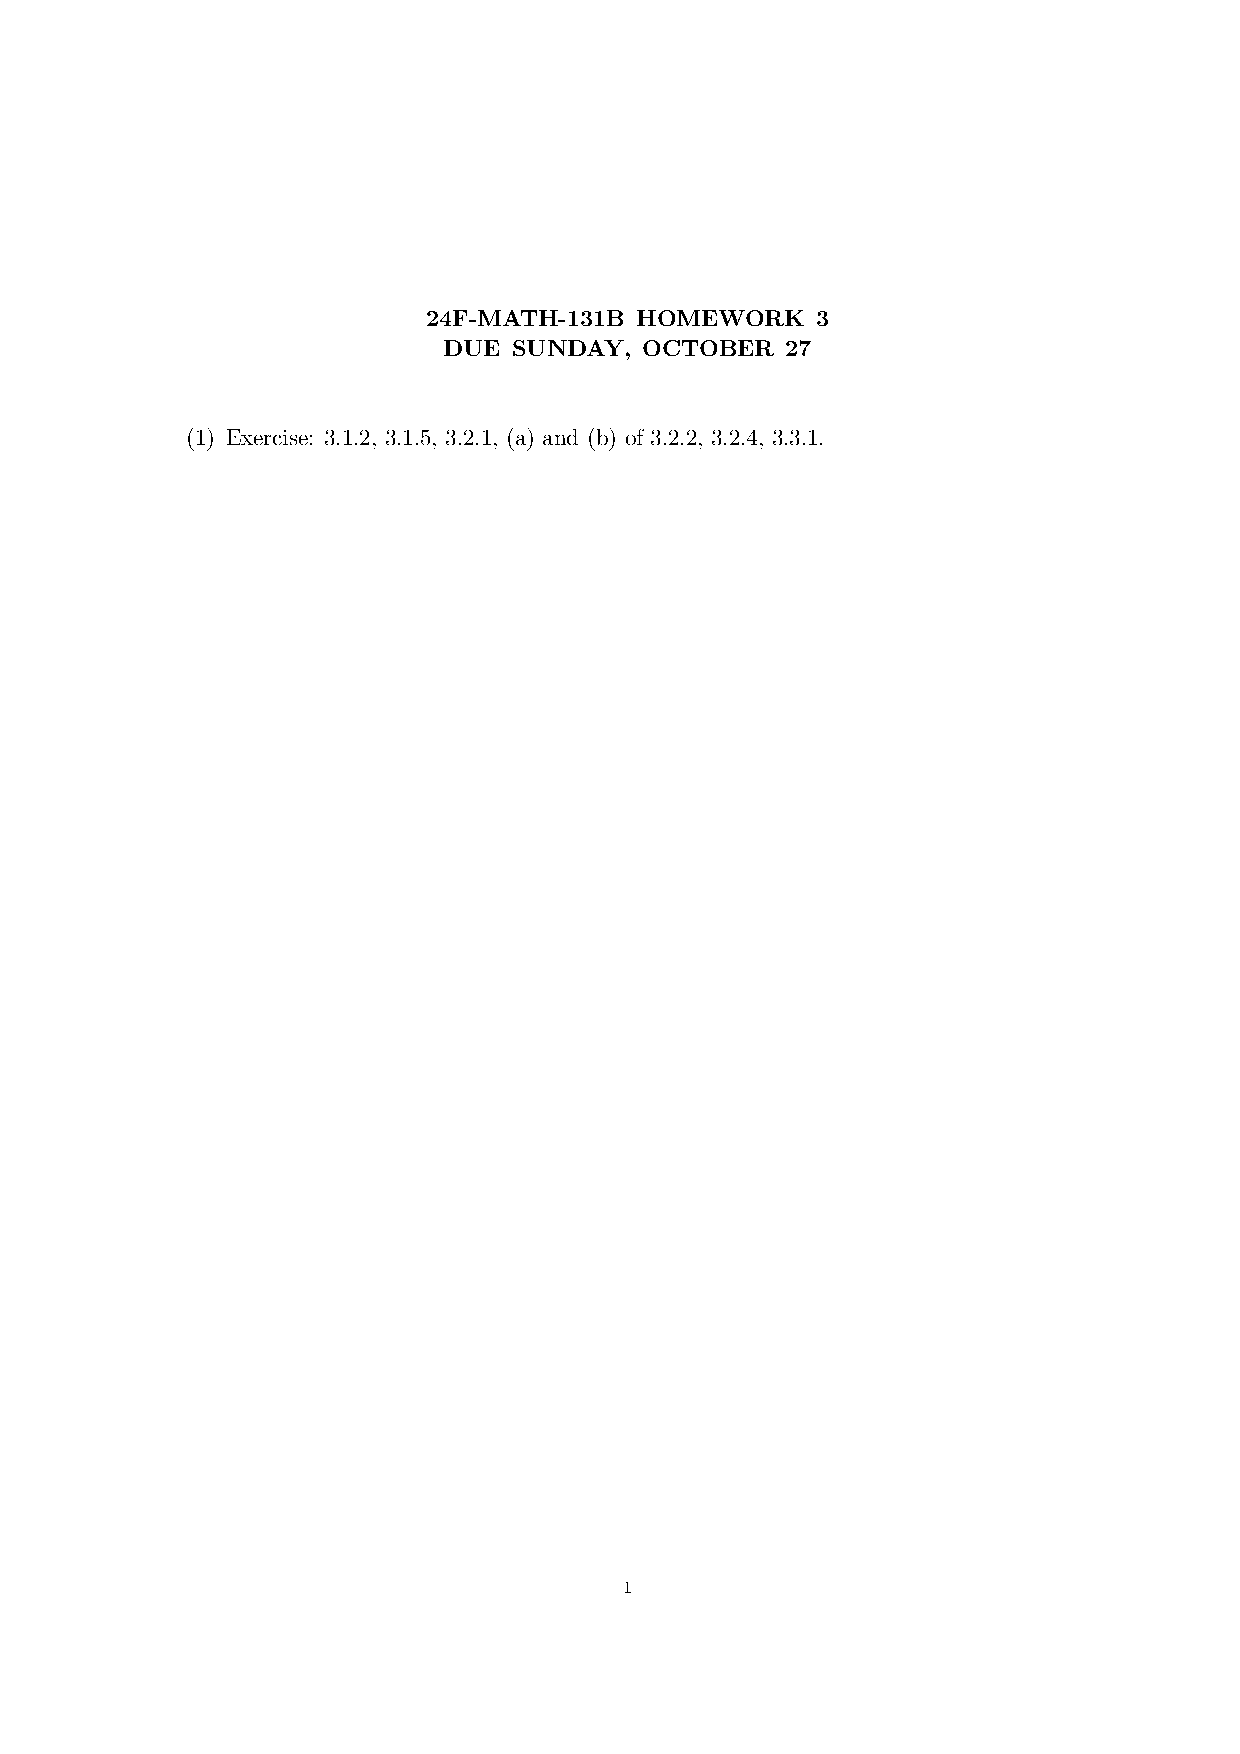
\includepdf[pages=-]{assignment.pdf}

\end{document}
